
\subsection{Ejercicios}
\begin{itemize}
 \item \textbf{Ejercicio 1 } Programar un tipo de tarea TaskConsola, que simulara una tarea interactiva.
La tarea debe realizar n llamadas bloqueantes, cada una de una duracion al azar 1 entre bmin
y bmax (inclusive). La tarea debe recibir tres parametros: n, bmin y bmax (en ese orden) que
seran interpretados como los tres elementos del vector de enteros que recibe la funcion.
\item \textbf{Ejercicio 2} Rolando, uno de los investigadores del departamento, utiliza su computadora
para correr un algoritmo muy complejo que hace un uso intensivo de la CPU por 100 ciclos
y no utiliza ninguna llamada bloqueante. Mientras corre su algoritmo suele poner su cancion
preferida y luego navegar por internet (estas tareas realizan 20 y 25 llamadas bloqueantes
respectivamente con una duracion variable entre 2 y 4 ciclos).\\
Escribir el lote de tareas que simule la situacion de Rolando. Ejecutar y graficar la simulacion
usando el algoritmo FCFS para 1 y 2 nucleos con un cambio de contexto de 4 ciclos.\\
Calcular la latencia de cada tarea en los dos graficos. Explicar que desventaja tendrıa Rolando
si debe mantener este algoritmo de scheduling y solo tiene disponible una computadora con un
nucleo (haga referencia a los graficos y a los calculos anteriores para justificar su explicacion).
\item \textbf{Ejercicio 3}Programar un tipo de tarea TaskBatch que reciba dos parametros: total cpu y
cant bloqueos. Una tarea de este tipo debera realizar cant bloqueos llamadas bloqueantes, en
momentos elegidos pseudoaleatoriamente. En cada tal ocasion, la tarea debera permanecer
bloqueada durante exactamente un (1) ciclo de reloj. \\
El tiempo de CPU total que utilice una
tarea TaskBatch debera ser de total cpu ciclos de reloj (incluyendo el tiempo utilizado para
lanzar las llamadas bloqueantes; no ası el tiempo en que la tarea permanezca bloqueada).
Explique la implementacion realizada y grafique un lote que utilice 3 tareas TaskBatch con
parametros diferentes y que corra con el scheduler FCFS.
\end{itemize}

\subsection{Resultados y Conclusiones}

\subsubsection[Resolución Ejercicio 1]{Ejercicio 1}

\indent Dada la simpleza del código, optamos por mostrar nuestra ximplementación, en vez de comentarlo detalladamente.\\
\indent Realizamos un ciclo de i < params[0], donde utilizamos la función dada por la catedra, uso\_IO a la cual le pasamos
el pid correspondiente y un entero ciclos que es el valor random obtenido entre $bmin$ y $bmax$. Esa función uso\_IO simula una llamada bloqueante.
\begin{center}
 \begin{verbatim}
                     ciclos = rand() % (params[2] - params[1] + 1) + params[1];
 \end{verbatim}

\end{center}

\indent A continuacion, el codigo mencionado:

\begin{verbatim}

                  void TaskConsola(int pid, vector<int> params) {
                       int i, ciclos;              
                       for (i = 0; i < params[0]; i++) {
                              ciclos = rand() % (params[2] - params[1] + 1) + params[1];  
                              uso_IO(pid, ciclos);
                       }
                  } 

\end{verbatim}

\subsubsection[Resolución Ejercicio 2]{Ejercicio 2}

CALCULAR LATENCIA!

\indent Para este punto, utilizamos el siguiente lote de tareas:
\begin{verbatim}
 
                                     TaskCPU 100
                                     TaskConsola 20 2 4
                                     TaskConsola 25 2 4


\end{verbatim}

\indent El mismo, presenta una tarea de uso intensivo $TaskCPU$ que dura 100 ticks, y otras dos interactivas, las cuales se
bloquean 20 y 25 ticks respectivamente con una duración de entre 2 y 4 tanto para la primera como la segunda.\\
A continuación, los respectivos gráficos de mediciones.


\vspace*{0.3cm} \vspace*{0.3cm}
  \begin{center}
 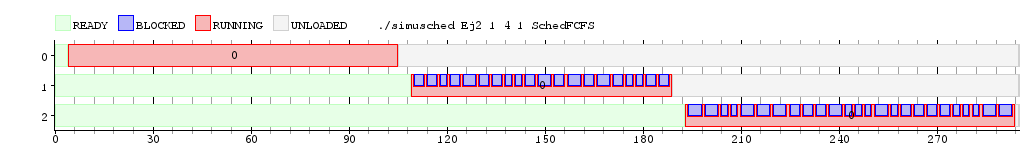
\includegraphics[scale=0.5]{./Test/ej2_1.png}
 { $Lote 1$ Scheduler FCFS - 1 core }
 \end{center}
  \vspace*{0.3cm}


\vspace*{0.3cm} \vspace*{0.3cm}
  \begin{center}
 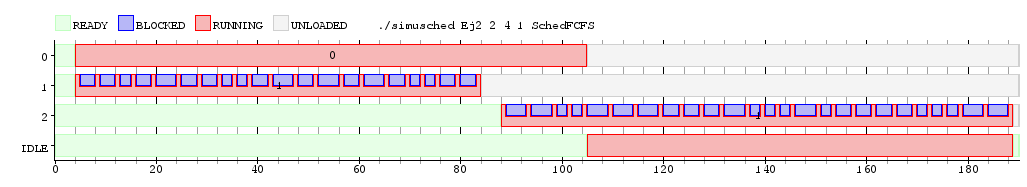
\includegraphics[scale=0.5]{./Test/ej2_2.png}
 { $Lote 1$ Scheduler FCFS - 2 core }
 \end{center}
  \vspace*{0.3cm}


\indent Debido a las tareas de tipo TaskConsola, se observa que en los dos casos la duración 
de cada bloqueo es distinta.\\
\indent A modo de análisis, se puede observar por medio de los gráficos como aumenta el paralelismo a mayor cantidad de núcleos. 
En este scheduler en particular, esto ayuda de gran manera al rendimiento del sistema, puesto que un núcleo podrá ejecutar otra tarea 
recién cuando haya terminado la anterior. Las consecuencias de este comportamiento son visibles en los 2 graficos. Agregando un core más, 
el tiempo que se tarda en ejecutar por completo todas las tareas de reduce casi a la mitad.\\

\subsubsection[Resolución Ejercicio 3]{Ejercicio 3}

\indent Al igual que con la tarea TaskConsola, mencionaremos nuestro implementación y por consiguiente  
explicaremos ciertos puntos de la misma.\\
 \begin{verbatim}
                       void TaskBatch(int pid, vector<int> params) {
                            int total_cpu = params[0];
                            int cant_bloqueos = params[1];
                            srand(time(NULL));
                            vector<bool> uso = vector<bool>(total_cpu);
                            for(int i=0;i<(int)uso.size();i++) 
                               uso[i] = false;
	                       for(int i=0;i<cant_bloqueos;i++) {
                                   int j = rand()%(uso.size());
                                   if(!uso[j])
                                      uso[j] = true;
                                   else
                                      i--; 
                                   }
                            for(int i=0;i<(int)uso.size();i++) {
                                if( uso[i] )
                                    uso_IO(pid,1); 
                                else
                                    uso_CPU(pid, 1); 
                               }
                            }
 \end{verbatim}

 \indent Para este tipo de tarea, creamos un vector de tamaño igual a $total_cpu$ el cual tendrá bool, ya sea true o false
 dependiendo del uso que se le de dentro de la tarea, ya sea uso\_IO o uso\_CPU. En caso de ser uso\_IO sera true, y sino false.\\
 Luego, utilizaremos un ciclo que irá desde 0 hasta el tamaño del vector y dependiendo el valor booleano, usará la funciones
 dadas por la catedra uso\_IO o uso\_CPU.\\
 
 
 ACA FALTARIA PROBAR UN LOTE DE TAREAS
 
  \begin{center}
  \textbf{Conclusiones}
 \end{center}


\indent \indent La diferencia entre los valores de quantum entre los casos 
se puede presumir a que cada vez que agregamos un núcleo aumentamos 
la posibilidad de una migración de la tareas.\\
\indent \indent En todos lo casos se observa la influencia negativa que proviene 
de elegir un quantum con valores pequeños.\\
\indent \indent Agregar núcleos de procesamiento mejora significativamente 
la performance de acuerdo a la métricas con las que
trabajamos, al permitir más procesamiento en pararelo y disminuyendo 
los waiting time de las tareas.\\
\indent \indent  Fijada una cantidad de núcleos puntual, aumentar el valor del
quantum también mejora la performance, igualmente, como vimos, a partir de cierto valor 
de quantum, las mejoras en la performance tienden a estabilizarse y dejan de ser 
muy significativas. 
Esto se produce a que las tareas con mas cantidad de bloqueos en 
algun momento dejan de consumir todo el quantum otorgado si este es aumentado en su valor.
